\documentclass[tikz,border=3pt]{standalone}
\usepackage[utf8]{inputenc}
\usepackage[T1]{fontenc}
\usepackage{lmodern}
\renewcommand{\familydefault}{\sfdefault}
\usepackage{sansmath}\sansmath
\usepackage{chemfig}
\usepackage{pgfplots}\pgfplotsset{compat=1.18,/pgf/number format/use comma,/pgf/number format/1000 sep={.}}
\usetikzlibrary{arrows.meta,calc,positioning,decorations.pathmorphing,patterns}
% paleta del sitio
\definecolor{nar}{HTML}{E8680C}\definecolor{narc}{HTML}{FFB35C}\definecolor{hielo}{HTML}{FFF3E8}
\definecolor{tinta}{HTML}{1D1D1F}\definecolor{gris}{HTML}{6E6E73}\definecolor{lila}{HTML}{7C5CF0}
\definecolor{azul}{HTML}{2F6FD6}\definecolor{menta}{HTML}{17A673}\definecolor{coral}{HTML}{E8342A}
\begin{document}
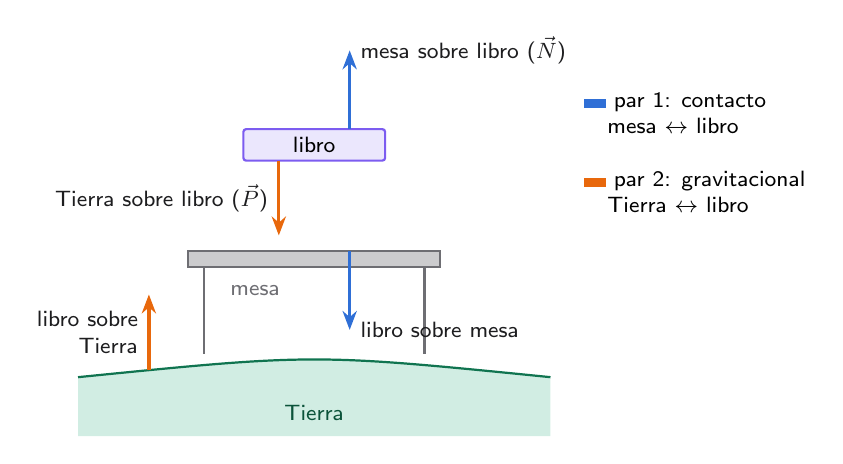
\begin{tikzpicture}[font=\footnotesize,>={Stealth[length=2.4mm]}]
% libro (separado de la mesa para ver las fuerzas)
\draw[thick,draw=lila,fill=lila!15,rounded corners=1pt] (-0.9,2.8) rectangle (0.9,3.2);
\node at (0,3.0) {libro};
\draw[->,very thick,azul] (0.45,3.2) -- (0.45,4.2) node[right,text=tinta] {mesa sobre libro ($\vec N$)};
\draw[->,very thick,nar] (-0.45,2.8) -- (-0.45,1.85) node[midway,left,text=tinta] {Tierra sobre libro ($\vec P$)};
% mesa
\fill[gris!35] (-1.6,1.45) rectangle (1.6,1.65);
\draw[thick,gris] (-1.6,1.45) rectangle (1.6,1.65);
\draw[thick,gris] (-1.4,1.45) -- (-1.4,0.35) (1.4,1.45) -- (1.4,0.35);
\node[gris] at (-0.75,1.15) {mesa};
\draw[->,very thick,azul] (0.45,1.65) -- (0.45,0.65) node[right,text=tinta] {libro sobre mesa};
% Tierra
\fill[menta!20] (-3.0,0.05) .. controls (0,0.35) .. (3.0,0.05) -- (3.0,-0.7) -- (-3.0,-0.7) -- cycle;
\draw[thick,menta!70!black] (-3.0,0.05) .. controls (0,0.35) .. (3.0,0.05);
\node[menta!50!black] at (0,-0.4) {Tierra};
\draw[->,very thick,nar] (-2.1,0.14) -- (-2.1,1.1) node[midway,left,text=tinta,align=right] {libro sobre\\Tierra};
% leyenda
\node[anchor=west,align=left] at (3.3,3.4) {\textcolor{azul}{\rule{8pt}{3pt}} par 1: contacto\\ \quad mesa $\leftrightarrow$ libro};
\node[anchor=west,align=left] at (3.3,2.4) {\textcolor{nar}{\rule{8pt}{3pt}} par 2: gravitacional\\ \quad Tierra $\leftrightarrow$ libro};
\end{tikzpicture}
\end{document}
